\section{\ON{} model}
\subsection{Selected vertices, propagators, and regulator insertions}\label{app:zerodONvpr}
\renewcommand{\FSk}{t}
In this appendix we will present the for \cref{sec:0dON} relevant two-point functions, regulator insertions, propagators, and vertices. 
Those are obtained by taking functional derivatives of the \eaa{} \eqref{eq:ansatz_effective_average_action} and evaluating the resulting expressions on the 
\qeom{}, \viz{} projecting on to $\varphi_{\eom{}}=\underline{\varphi} \equiv(0,\ldots,0,\sigma)$:
\begin{align}
\big(A_{\ldots}^{\ldots}\big)_{\varphi=\varphi_\eom{}=\underline{\varphi}}\equiv \underline{A}_{\ldots}^{\ldots}\,.
\end{align}
We will mark uncontracted, external indices with an underscore, in the spirit of \cref{subsec:higherOrderFlowEquations}, and the involved and $SO(N-1)$ flavor indices are $i\in{1,\ldots,N-1}$.
Note that traces in flavour space lead to the $N - 1$ multiplicity of the pion loop contributions, \cf{} \cref{eq:flow_equation_effective_potential}.
\bigskip

The non-vanishing two-point functions are
\begin{subequations}\label{eq:SON0dGamma2}
\begin{alignat}{2}
\FSvertexArg{\FSeaaEoM}{{\pi} {}_{\underline{j}},{\pi} {}_{\underline{i}}}&\equiv \begin{gathered}\raisebox{-3pt}{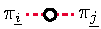
\includegraphics{appendix/diagrams/SU2model0d-Gamma2pp.pdf}}\end{gathered} &&= \delta_{\underline{i},\underline{j}} \tfrac{\FScoupling{U}{1}{\sigma}}{\sigma } = \delta_{\underline{i},\underline{j}} \tfrac{u(t,\sigma)}{\sigma}  \, , \\[1em] 
\FSvertexArg{\FSeaaEoM}{\sigma,\sigma}&\equiv \begin{gathered}\raisebox{-3pt}{
\includegraphics{appendix/diagrams/SU2model0d-Gamma2ss.pdf}}\end{gathered} &&=\FScoupling{U}{2}{\sigma} = \partial_\sigma u(t,\sigma)\,.
\end{alignat}
\end{subequations}

The regulator insertions \dash{} marked as usual with a crossed circle ($\otimes$) \dash{} are given by
\begin{subequations}\label{eq:SON0ddtR}
\begin{alignat}{2}
\partial_t\FSregulatorArg{\FSREoM}{{\pi} {}_{\underline{j}},{\pi} {}_{\underline{i}}}&\equiv \begin{gathered}\raisebox{-3pt}{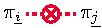
\includegraphics{appendix/diagrams/SU2model0d-Rpp.pdf}}\end{gathered} &&= \delta_{\underline{i},\underline{j}} \partial_t r(t) \, , \\[1em] 
\partial_t\FSregulatorArg{\FSREoM}{\sigma,\sigma}&\equiv \begin{gathered}\raisebox{-3pt}{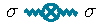
\includegraphics{appendix/diagrams/SU2model0d-Rss.pdf}}\end{gathered} &&=\partial_t r(t)\,,
\end{alignat}
\end{subequations}
and follow directly from \cref{eq:0dONR}.

Splitting radial and transversal modes in the unified propagator \eqref{eq:0dONG} leads to 
\begin{subequations}\label{eq:SON0dG}
\begin{alignat}{2}
\FSpropagatorArg{\FSGEoM}{{\pi} {}_{\underline{j}},{\pi} {}_{\underline{i}}}&= \begin{gathered}\raisebox{-3pt}{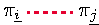
\includegraphics{appendix/diagrams/SU2model0d-Gpp.pdf}}\end{gathered} &&= \frac{1}{r_b(t)+u(t,\sigma)/\sigma} \delta_{\underline{i},\underline{j}}\, , \\[1em] 
\FSpropagatorArg{\FSGEoM}{\sigma,\sigma}&= \begin{gathered}\raisebox{-3pt}{
\includegraphics{appendix/diagrams/SU2model0d-Gss.pdf}}\end{gathered} &&= \frac{1}{r_b(t)+\partial_\sigma u(t,\sigma)}\,,
\end{alignat}
\end{subequations}
for the pion- and sigma-propagator\footnote{%
	The term ``propagator'' is of course misleading for a \qft{} in a single point, where ``propagation'' in the true sense of the word is not possible.
	Nevertheless, we again adopt the notation from higher-dimensional \qft{} and statistical mechanics for the zero-dimensional analog expressions.
} respectively.

The flow for the sigma-one-point function in \cref{eq:0dON1pt} includes the following vertices,
\begin{subequations}\label{eq:SON0dV}
\begin{alignat}{2}
\FSvertexArg{\FSeaaEoM}{\sigma}&=\begin{gathered}\raisebox{-3pt}{
\includegraphics{appendix/diagrams/SU2model0d-V0001.pdf}}\end{gathered}&&=\FScoupling{U}{1}{\sigma}=u(t,\sigma)\,,\\ 
\FSvertexArg{\FSeaaEoM}{{\pi} {}_{\underline{j}},{\pi} {}_{\underline{i}},\sigma}&=\begin{gathered}\raisebox{-6pt}{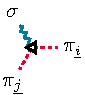
\includegraphics{appendix/diagrams/SU2model0d-V0021.pdf}}\end{gathered}&&=\partial_{\sigma}\,\Big[\frac{\FScoupling{U}{1}{\sigma}}{\sigma }\Big]\delta_{\underline{i},\underline{j}} =\partial_\sigma \big[ \tfrac{1}{\sigma} \, u ( t, \sigma ) \big] \delta_{\underline{i},\underline{j}}\,,\\ 
\FSvertexArg{\FSeaaEoM}{\sigma,\sigma,\sigma}&=\begin{gathered}\raisebox{-6pt}{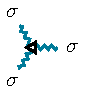
\includegraphics{appendix/diagrams/SU2model0d-V0003.pdf}}\end{gathered}&&=\FScoupling{U}{3}{\sigma} = \partial_\sigma^2 u(t,\sigma)\,.
\end{alignat}
\end{subequations}

\renewcommand{\FSk}{k}

\subsection{Numerical derivatives}
\begin{disclaimer}
	This appendix has been copied from App. A of \ccite{zerod1} with only small adaptations to the presentation in this thesis.
\end{disclaimer}
Throughout \cref{sec:0dON,subsec:0dO1Entropy,subsec:0dLargeN} we need to extract the \ipi{} vertex functions $\Gamma^{(2n)}_{\varphi_{i_1} \cdots \varphi_{i_{2n}}}$ at the physical point $\sigma = 0$ from the \ir{} results of the \frg{} flows (or respectively the coefficients $\Gamma^{(2n)}$, which contain the same information).
To this end, we compute numerical derivatives of the discrete values of the derivative of the effective potential $u ( t_\mathrm{IR}, \sigma ) = \partial_\sigma U ( t_\mathrm{IR}, \sigma )$, which were calculated via the \fv{} method.
In this work, the following \fd{} approximations~\cite{Fornberg1988,abramowitz+stegun} are used,
\begin{align}
	f^{(1,2)}_{i , \mathrm{c}} = \, & \frac{- f_{i - 1} + f_{i + 1}}{2 \, \Delta x} + \order ( \Delta x^2 ) \, ,		\label{eq:derivative_1_central_error_2}
	\\
	f^{(1,4)}_{i , \mathrm{c}} = \, & \frac{f_{i - 2} - 8 \, f_{i - 1} + 8 \, f_{i + 1} - f_{i + 2}}{12 \, \Delta x} + \order ( \Delta x^4 ) \, ,		\label{eq:derivative_1_central_error_4}
	\\
	f^{(1,2)}_{i , \mathrm{f}}  = \, & \frac{- 3 \, f_i + 4 \, f_{i + 1} - f_{i + 2}}{2 \, \Delta x} + \order ( \Delta x^2 ) \, ,		\label{eq:derivative_1_forward_error_2}
	\\
	f^{(3,2)}_{i , \mathrm{c}} = \, & \frac{- f_{i - 2} + 2 \, f_{i - 1} - 2 \, f_{i + 1} + f_{i + 2}}{2 \, \Delta x^3} + \order ( \Delta x^2 ) \, ,		\label{eq:derivative_3_central_error_2}
	\\
	f^{(3,4)}_{i , \mathrm{c}} = \, & \frac{f_{i - 3} - 8 \, f_{i - 2} + 13 \, f_{i - 1} - 13 \, f_{i + 1} + 8 \,  f_{i + 2} - f_{i + 3}}{8 \, \Delta x^3} + \order ( \Delta x^4 ) \, ,		\label{eq:derivative_3_central_error_4}
	\\
	f^{(3,2)}_{i , \mathrm{f}} = \, & \frac{- 5 \, f_{i} + 18 \, f_{i + 1} - 24 \, f_{i + 2} + 14 \, f_{i + 3} - 3 \, f_{i + 4} }{2 \, \Delta x^3} + \order ( \Delta x^2 ) \, ,		\label{eq:derivative_3_central_error_1}
	\\
	f^{(5,2)}_{i , \mathrm{c}} = \, & \frac{- f_{i - 3} + 4 \, f_{i - 2} - 5 \, f_{i - 1} + 5 \, f_{i + 1} - 4 \,  f_{i + 2} + f_{i + 3}}{2 \, \Delta x^5} + \order ( \Delta x^2 ) \, ,		\label{eq:derivative_5_central_error_2}
	\\
	f^{(5,4)}_{i , \mathrm{c}} = \, & \frac{f_{i - 4} - 9 \, f_{i - 3} + 26 \, f_{i - 2} - 29 \, f_{i - 1} + 29 \, f_{i + 1} - 26 \,  f_{i + 2} + 9 \, f_{i + 3} - f_{i + 4} }{6 \, \Delta x^5} + \order ( \Delta x^4 ) \, ,		\label{eq:derivative_5_central_error_4}
\end{align}
where $f_i \equiv f ( x_i )$, $f^{(n,m)}$ denotes the \ith{n} derivative of $f$ to order $ \order ( \Delta x^m )$, and the subscripts c/f stand for central/forward stencil approximations.
The scaling order $m$ of the error is indicated by $\order(\Delta x^m)$.
In our numerical implementation, the central-scheme approximations are further simplified by exploiting the antisymmetry property $u ( t, - \sigma ) = - u ( t, \sigma )$ of the derivative of the effective potential.
In consequence, the central stencils are effectively forward stencils.
Furthermore, at the same order of accuracy, the anti-symmetrized central stencils need one point less than the actual forward stencils of same error order of accuracy.
In \cref{fig:sc_i_on_n_400_xmax_10_lambda_1e6_tir_60_flow_errors} we find that this property singles out the central stencils as the most favorable choice, because the accumulation of errors in the derivative stencil, which originally derive from the numerical solution of the flow equation, can be reduced this way, by including as few points as possible in the numerical derivative approximations.

We stress that the use of low-order finite-difference approximations to the derivative is only justified because the effective \ir{} potential $U ( t_\mathrm{IR}, \sigma )$ has to be smooth, which is discussed at length in App. B of \ccite{zerod1}.
For higher-dimensional models, the use of finite-difference approximations to extract information from the \ir{} effective potential $U ( t_\mathrm{IR}, \sigma )$ might not always be justified due to the possibility of non-analyticities in the vicinity of the physical point, where the \ipi{} \nptFunctions{} have to be calculated. Further investigation is needed.

\subsection{Additional expressions for the \ON{} model in the \texorpdfstring{$N\rightarrow\infty$}{infinite-N} limit}
\begin{disclaimer}
	This appendix is compiled from Apps. A\dash{}D of \ccite{zerod3} with only minor adaptations to the presentation in this thesis.
\end{disclaimer}

\subsubsection{Analytical solution for the instructive toy model}
\label{app:RP_integrals}
Within this appendix we present results for the integral $I_n^N [ V ]$ of \cref{eq:In_largeN} for the potential \eqref{eq:RP_Vofy},
\begin{align}
	I_n^N [ V ] =& \, N^{- ( \frac{N}{2} + n )} \, \Big( \Gamma \big( \tfrac{N}{2} + n \big) - \Gamma \big( \tfrac{N}{2} + n, 2 N \big) + \eu^{6 N ( a + 1 )} \, \Gamma \big( \tfrac{N}{2} + n, 8 N \big)\, +\notag\\
	&\qquad\qquad+( - a )^{- ( \frac{N}{2} + n )} \, \eu^{- 2 N ( a + 1 )}\big[ \Gamma \big( \tfrac{N}{2} + n, - 2 N a \big) - \Gamma \big( \tfrac{N}{2} + n, - 8 N a \big) \big] \Big) \, ,		\label{eq:InNV_a0}
\end{align}
and in the special case $a = 0$,
	\begin{align}
		 I_n^N [ V ] 	= &\,  N^{- ( \frac{N}{2} + n )} \, \Bigg[ \Gamma \big( \tfrac{N}{2} + n \big) - \Gamma \big( \tfrac{N}{2} + n, 2 N \big)
 + \eu^{6 N} \, \Gamma \big( \tfrac{N}{2} + n, 8 N \big)\, + \notag\\
&\qquad\qquad\qquad\qquad\qquad\qquad\qquad\qquad\qquad+\eu^{-2 N} \, \frac{\big( 4^{\frac{N}{2} + n} - 1 \big) \, ( 2 N )^{\frac{N}{2} + n}}{\frac{N}{2} + n} \Bigg] \, ,  \label{eq:InNV}
	\end{align}
where 
\begin{align}
	&	\Gamma ( a, z ) \equiv \int_{z}^{\infty} \dif t \, t^{a - 1} \, \eu^{-t} \, ,	\qquad	\Gamma ( z ) \equiv \Gamma ( z, 0 ) \, ,
\end{align}
is the (incomplete) gamma function. To determine the leading order contribution to $\langle ( \vec{\phi}^{\, 2} )^n \rangle$ in the limit ${N \rightarrow \infty}$ assuming finite $n$, we employ the asymptotic series, see, \eg{}, Secs.~6.1.41 and 6.5.32 of Ref~\cite{abramowitz+stegun} or Secs.~5.11 and 8.11 of \ccite{NIST:DLMF},
\begin{subequations}\label{eq:GammaFktSeries}
\begin{align}
	\Gamma ( z ) = \, & \eu^{-z} \, \sqrt{\tfrac{2 \piu }{z}} \, z^z \, \big( 1 + \tfrac{1}{12 z} + \tfrac{1}{288 z^2} + \ldots \big) \, ,	\\
	\Gamma ( a, z ) = \, & \eu^{-z} \, z^{a - 1} \, \big( 1 + \tfrac{a-1}{z} + \tfrac{( a - 2 ) ( a - 1 )}{z^2} + \ldots \big) \, ,	
\end{align}
\end{subequations}
valid for large real $z$ and in case of $\Gamma ( a, z )$ for $a \simeq \order ( z )$~\cite{Temme1975}.

For $a = 0$ we find
\begin{align}
	\lim_{N \rightarrow \infty} \tfrac{1}{N^n} \, \big\langle ( \vec{\phi}^{\, 2} )^n \big\rangle = \lim_{N \rightarrow \infty} \frac{2^n I_n^N [ V ]}{I_0^N [ V ]} \bigg|_{a = 0} = 1 \, ,
\end{align}
while for $a > 0$
\begin{subequations}\label{eq:RP_phi2_th}
\begin{align}	
	\lim_{N \rightarrow \infty} \tfrac{1}{N^n} \, \big\langle ( \vec{\phi}^{\, 2} )^n \big\rangle =	&\,  \lim_{N \rightarrow \infty} \frac{2^n I_n^N [ V ]}{I_0^N [ V ]}= 
	\\[.2em]
	=&\, \lim_{N \rightarrow \infty} \frac{17 \, \eu^{6 N a} \, 16^{\frac{N}{2} + n} + 256 \, \sqrt{N \piu} \, \eu^{\frac{n^2}{N} + \frac{3 N}{2}}}{17 \, \eu^{6 N a} \, 4^N + 256 \, \sqrt{N \pi} \, \eu^{\frac{3 N}{2}}} = \label{eq:RP_phi2_thA}	
	\\[.2em]
	= &\, 
	\begin{cases}
		1		&	\text{for} \quad a \leq a_\mathrm{c} \, ,
		\\
		16^n	&	\text{for} \quad  a>a_\mathrm{c} \, ,
	\end{cases}		\label{eq:RP_phi2_thB}	
\end{align}
\end{subequations}
where ${a_\mathrm{c}\equiv\tfrac{1}{4} - \tfrac{1}{3} \ln ( 2 ) \simeq 0.018951}$. For $a > a_\mathrm{c}$ the first terms in the denominator and numerator of \cref{eq:RP_phi2_thA} dominate, while for $a < a_\mathrm{c}$ the second terms dominate. For $a=a_\mathrm{c}$ \cref{eq:RP_phi2_thA} can be simplified ultimately to $\eu^{\frac{n^2}{N}}$ under the limit $N\rightarrow\infty$ and thus yielding $1$ in the limit.

\subsubsection{Saddle-point expansion at large \texorpdfstring{$N$}{N}}
\label{app:saddle_point_app}

In this appendix we present the so-called saddle-point expansion for integrals of the type
	\begin{align}
		I^N [ f, g ] \equiv \int_{0}^{\infty} \dif y \, g ( y ) \, \eu^{- N f ( y )} \, .	\label{eq:SPapp_Idef}
	\end{align}
Assuming that $f(y)$ has a unique global minimum at $y_0$ and further assuming analyticity (expandability to arbitrary order) of $f ( y )$ and also $g ( y )$ in $y_0$, it is possible to derive an asymptotic series of $I^N [ f, g ]$ for large $N$ if the series expansions of $f ( y )$ and $g ( y )$ around $y_0$ grow like polynomials. We focus here on the one-dimensional integral \eqref{eq:SPapp_Idef} see, \eg{}, \ccite{Arfken:2005} for further details and generalizations.

For large $N$ the integrand of \cref{eq:SPapp_Idef} is peaked around $y_0$ and we therefore consider an expansion around $y_0$ using the computational coordinate $z$ defined by
	\begin{align}
		y = y_0 + \tfrac{z}{\sqrt{N}} \, .
	\end{align}
We proceed with the computation of $I^N [ f, g ]$ at large $N$:
\begin{subequations}\label{eq:SPapp}
\begin{align}	
	I^N [ f, g ] =\,& \int_{0}^{\infty} \dif y \, g ( y ) \, \eu^{- N f ( y )} =	 
	\\
	= \, & \tfrac{1}{\sqrt{N}} \int_{- y_0 \sqrt{N}}^{\infty} \dif z \, g \big( y_0 + \tfrac{z}{\sqrt{N}} \big) \, \exp \big[ - N f \big( y_0 +\tfrac{z}{\sqrt{N}} \big) \big] =		\label{eq:SPapp_Ishift}
	\\
	= \, & \tfrac{1}{\sqrt{N}} \int_{- y_0 \sqrt{N}}^{\infty} \dif z \, g \big( y_0 + \tfrac{z}{\sqrt{N}} \big) \, \exp \Big[ - N f^{(0)} - \tfrac{1}{2} \, f^{(2)} \, z^2 -\notag\\[.1em]
	&\qquad\qquad\qquad\qquad\qquad\qquad- \tfrac{1}{6 \sqrt{N}} \, f^{(3)} \, z^3 - \tfrac{1}{24 N} \, f^{(4)} \, z^4 - \order ( z^5 ) \Big] \simeq	 
	\\[.2em]
	\simeq \, & \eu^{- N f^{(0)}} \tfrac{1}{\sqrt{N}} \int_{-\infty}^{+\infty} \dif z \, \eu^{- \tfrac{1}{2} f^{(2)} z^2} \, g \big( y_0 + \tfrac{z}{\sqrt{N}} \big) \, \Big( 1 - \tfrac{1}{6 \sqrt{N}} \, f^{(3)} \, z^3 +\notag\\[.1em]
	&\qquad\qquad\qquad\qquad\qquad+\tfrac{1}{72 N} \, \big[ ( f^{(3)} )^2 \, z^6 - 3 \, f^{(4)} \, z^4 \big] + \order \big( N^{-\tfrac{3}{2}} \big) \Big) =	 
	\\[.2em]
	= \, & \eu^{- N f^{(0)}} \tfrac{1}{\sqrt{N}}\int_{-\infty}^{+\infty} \dif z \, \eu^{-\tfrac{1}{2} f^{(2)} z^2} \Big( g^{(0)} + \tfrac{1}{\sqrt{N}} \, \big[ g^{(1)} - \tfrac{1}{6} \, g^{(0)} \, f^{(3)} \, z^2 \big] \, z +		\notag\\
	& \qquad\qquad\qquad\qquad\qquad + \tfrac{1}{N} \, \big[ \tfrac{1}{2} \, g^{(2)} - \tfrac{1}{6} \, g^{(1)} \, f^{(3)} \, z^2 + \tfrac{1}{72} \, g^{(0)} \, ( f^{(3)} )^2 \, z^4 - \notag\\[.1em]
	& \qquad\qquad\qquad\qquad\qquad -\tfrac{1}{24} \, g^{(0)} \, f^{(4)} \, z^2 \big] \, z^2 + \order \big( N^{-\tfrac{3}{2}} \big) \Big) =	\label{eq:SPapp_int}	
	\\[.2em]
	= \, & \eu^{- N f^{(0)}} \sqrt{\tfrac{2 \piu}{N f^{(2)}}} \, \sum_{i = 0}^{\infty} C_i [ f, g ] \, N^{-i} \, ,	 \label{eq:SPapp_Isp}
\end{align}
\end{subequations}
where we abbreviated \ith{n} derivatives of $f$ and $g$ evaluated at $y_0$ with superscripts $(n)$.
In the preceding set of equalities we first expanded the exponent in powers of $N$ after switching to the coordinate $z$.
We split of the contributions of $\order ( N^1 )$ and $\order ( N^0 )$ in the exponent and then expanded the exponential in an asymptotic series in $N$, while shifting the lower integration bound\footnote{%
	Since we are interested in an asymptotic power series for large $N$ shifting the lower integration bound in line \eqref{eq:SPapp_Ishift} is valid since contributions stemming from this shift decay exponentially and as such faster than any power.
}.
Afterwards, we continued by expanding $g$ and collecting terms of $\order ( N^{- \tfrac{n}{2}} )$.
Ultimately, we were left with a sum over Gaussian integrals of $\order ( N^{-n} )$ and vanishing contributions of odd integrands of $\order ( N^{- \tfrac{2 n + 1}{2}} )$ in \cref{eq:SPapp_int} and performed those integrals, which left us with the desired power series \eqref{eq:SPapp_Isp} with coefficients $C_i [ f, g ]$ of $\order ( N^0 )$, \eg{},
\begin{subequations}\label{eq:SappCi}
\begin{align}
	C_0 [ f, g ] = \, & g^{(0)} \, ,\\
	C_1 [ f, g ] = \, & \frac{g^{(2)}}{2 f^{(2)}} - \frac{g^{(1)} f^{(3)}}{2 ( f^{(2)} )^2} +\frac{5 g^{(0)} ( f^{(3)} )^2}{24 ( f^{(2)} )^3} - \frac{g^{(0)} f^{(4)}}{8 ( f^{(2)} )^2} \, .
\end{align}
\end{subequations}
The computation of higher-order coefficients is straightforward and tedious by hand, but is easy to implement in computer algebra systems like \WAMXIIwR{}, \cf{} the digital auxiliary file~\cite{Steil:2023zeroDlargeN}.

The presented saddle-point expansion of $I^N [ f, g ]$ can be used in combination with \cref{eq:ON_expectation_value_largeN} for a large-$N$ expansion of the expectation values $\langle ( \vec{\phi}^{\, 2} )^n \rangle$
\begin{align}
	\tfrac{1}{N^n} \, \langle ( \vec{\phi}^{\, 2} )^n \rangle = \, & \frac{2^n I^N [ V ( y ) - \tfrac{1}{2} \ln ( y ), y^{n - 1} ]}{I^N [ V ( y ) - \tfrac{1}{2} \ln ( y ), y^{-1} ]} =\nonumber\\
	= \, & 2^n \, y_0^n + \frac{1}{N} \, \frac{n \, 2^n \, y_0^n \big[ 2 ( n - 3 ) \, y_0^2 \, V^{(2)} ( y_0 ) + n - 2 y_0^3 \, V^{(3)} ( y_0 ) - 1 \big]}{\big[ 2 y_0^2 \, V^{(2)} ( y_0 ) + 1 \big]^2} + \order ( N^{-2} ) \, ,\label{eq:SPapp_series}
\end{align}
which is valid for $V(y)-\tfrac{1}{2}\ln(y)$ which are analytic around their respective unique global minimum $y_0$.
Corresponding expressions for the \ipi{} correlation functions can be derived using the relations between $\Gamma^{(n)}$ and $\langle ( \vec{\phi}^{\, 2} )^n \rangle$, see, \eg{}, Eqs.~(70)-(75) of \ccite{Koenigstein:2021syz} or \ccite{Keitel:2011pn}.

\subsubsection{Results from the method of characteristics}
\label{app:method_of_characteristics}
In this appendix we derive the expressions for the characteristic curves of \cref{eq:frg_flow_Ninf_x} and \eqref{eq:frg_flow_Ninf_y} using the method of characteristics and to be specific the Lagrange–Charpit Eqs.~\eqref{eq:MoC_odes} introduced in \cref{subsec:MoC}.

We proceed with the solution of the characteristic Eqs.~\eqref{eq:MoC_odes} for the \frg{} flow \cref{eq:frg_flow_Ninf_x} and \eqref{eq:frg_flow_Ninf_y} of the zero-dimensional $O(N)$~model in the limit $N \rightarrow \infty$.
Since the equations in $x$ and $y$ are related by the coordinate transformation ${y = \tfrac{1}{2} \, x^2}$, the solutions and also characteristics curves are directly related.
For simplicity we solve the characteristic equations for the flow equation \eqref{eq:frg_flow_Ninf_y} in the rescaled invariant $y$ and then compute the corresponding curves in $x$ using the coordinate transformation.
A direct solution of the characteristic equations for the flow equation \eqref{eq:frg_flow_Ninf_x} in $x$ is also possible and shares a lot of computations with the slightly simpler computation in $y$.
After performing the $y$ derivative in \cref{eq:frg_flow_Ninf_y} comparing coefficients with \cref{eq:MoC_pde} yields for the Eqs.~\eqref{eq:MoC_odes} explicitly
\begin{subequations}\label{eq:MoC_ode_y}
\begin{align}	
	\frac{\partial t ( \tau )}{\partial \tau} = \, & 1 \,,	\label{eq:MoC_ode_y_1}
	\\* % no page break
	\frac{\partial y ( \tau )}{\partial \tau} = \, & - \frac{\Lambda \, \eu^{- t ( \tau )}}{2 \, [ \Lambda \, \eu^{- t ( \tau )} + v ( \tau ) ]^2} \, ,	\label{eq:MoC_ode_y_2}
	\\* % no page break
	\frac{\partial v ( \tau )}{\partial \tau} = \, & 0 \, ,	\label{eq:MoC_ode_y_3}
\end{align}
\end{subequations}
with the \uv{} \ics{}
\begin{subequations}
\begin{align}
	t ( \tau = 0 ) = \, & 0 \, ,\\*[.1em] % no page break
	y ( \tau = 0 ) = \, & y_0 \geq 0 \, ,\\*[.1em] % no page break
	v ( \tau = 0 ) = \, & v ( 0, y_0 ) \, ,
\end{align}
\end{subequations}
specifying the characteristic curves. The \odes{} for $t(\tau)$ and $v(\tau)$ decouple and can be trivially integrated 
\begin{align}
	t ( \tau )= \, & \tau \, ,		\label{eq:MoC_toftau}
	\\
	v ( \tau ) = \, & v ( 0, y_0 ) \, .		\label{eq:MoC_vyoftau}
\end{align}
Due to the direct equivalence of $t$ and $\tau$ we continue by using the \rgtime{} $t$ as the curve-parameter in the following. The \ode{} \eqref{eq:MoC_ode_y_2} for $y(\tau)$ is independent of $y$ itself and can be integrated directly after inserting the solutions \eqref{eq:MoC_toftau} and \eqref{eq:MoC_vyoftau} for $t$ and $v$. The solution for $y ( t )$ follows as
	\begin{subequations}\label{eq:MoC_yoftau}
	\begin{align}
		y ( t ) = \, & y_0 - \int_0^t \dif \tau \, \frac{\Lambda \, \eu^{- \tau}}{2 \, [ \Lambda \, \eu^{- \tau} + v ( 0, y_0 ) ]^2} =
		\\* % no page break
		= \, & y_0 - \frac{1}{2 \, [ \Lambda \, \eu^{-t} + v ( 0, y_0 ) ]} + \frac{1}{2 \, [ \Lambda + v ( 0, y_0 ) ]} \, .	
	\end{align}
	\end{subequations}
Using the coordinate transformation ${y = \tfrac{1}{2} \, x^2}$ and the associated relation for the first derivative ${\partial_y V ( t, y ) = \tfrac{1}{x} \, \partial_x V ( t, x )}$ we can compute the characteristic curves $x ( t )$ and $v ( t )$ for the flow \cref{eq:frg_flow_Ninf_x} from \cref{eq:MoC_yoftau} and \eqref{eq:MoC_vyoftau},
	\begin{align}
		x ( t ) = \, & \pm \sqrt{2 y ( t )} =	\,\pm \sqrt{x_0^2 - \frac{1}{\Lambda \, \eu^{- t} + \tfrac{v ( 0, x_0 )}{x_0}} + \frac{1}{\Lambda + \tfrac{v ( 0, x_0 )}{x_0}} } \, ,	\label{eq:MoC_xoftau}
		\\
		v ( t ) = \, & \tfrac{v ( 0, x_0 )}{x_0} \, x ( t ) \, .\label{eq:MoC_vxoftau}
	\end{align}
A particularity of the flow equation in $x$ is that the conserved quantity $v ( t, x )$ (the derivative $\partial_x V ( t, x )$) is not constant along the characteristics, $\tfrac{\dif v}{\dif t} \neq 0$, due to the contribution stemming from $x ( t )$ in \cref{eq:MoC_vxoftau}.	

\subsubsection{Rankine-Hugoniot condition and shock position}
\label{app:rankine-hugoniot_condition_and_shock_position}

The Riemann problems posed by the \ic{} \eqref{eq:RP_vofy} with the flow \cref{eq:frg_flow_Ninf_y} include a shock discontinuity in the \uv{} ($t = 0$) at $y = 2$, since $v ( 2^{-} ) > v ( 2^{+} )$ and $G [ t, v ] < 0$. For a discussion see \cref{paragraph:largeNchars}.
This appendix is dedicated to the computation of the position of the shock as a function of flow time $t$ using the Rankine-Hugoniot condition~\cite{Rankine:1870,Hugoniot:1887} introduced in \cref{subsec:MoC}.
A computation in the invariant $y$ for a structurally identical flow equation and \ic{} can be found in App.~C.1 of \ccite{Grossi:2019urj}.
We present a derivation for the complementary problem \dash{} \ic{}  \eqref{eq:RP_vofx} with the flow \cref{eq:frg_flow_Ninf_x} \dash{} in $x$ for the sake of completeness in the following.\bigskip

Assume that there is a single shock wave (discontinuity) at the position $\xi_\mathrm{s} ( t )$ between ${ x_\mathrm{L} ( t ) < \xi_\mathrm{s} ( t ) < x_\mathrm{R} ( t ) }$. Integration over the conservation law \eqref{eq:frg_flow_Ninf_x} yields
	\begin{align}
	 \int_{x_\mathrm{L} ( t )}^{x_\mathrm{R} ( t )} \dif x \, \partial_t v ( t, x ) =& \,  \int_{x_\mathrm{L} ( t )}^{x_\mathrm{R} ( t )} \dif x \, \dod{}{x} F [ t, x , v ( t, x ) ] =\nonumber\\*[.2em] % no page break
	=&\,- \big( F [ t, x_\mathrm{R} ( t ), v ( t, x_\mathrm{R} ( t ) ) ] - F [ t, x_\mathrm{L} ( t ), v ( t, x_\mathrm{L} ( t ) ) ] \big)		\, . 
	\end{align}
For the \lhs{}, we split the integral about the shock $\xi_\mathrm{s} ( t )$
	\begin{align}
		\int_{x_\mathrm{L} ( t )}^{x_\mathrm{R} ( t )} \dif x \, \partial_t v ( t, x )\nonumber
		= \, & \int_{x_\mathrm{L} ( t )}^{\xi_\mathrm{s} ( t )} \dif x \, \partial_t  v ( t, x ) + \int_{\xi_\mathrm{s} ( t )}^{x_\mathrm{R} ( t )} \dif x \, \partial_t  v ( t, x ) =		\nonumber\\*[.2em] % no page break
		= \, & - v ( t, \xi_\mathrm{s} ( t) ) \, \partial_t \xi_\mathrm{s} ( t ) + v ( t, x_\mathrm{L} ( t ) ) \, \partial_t x_\mathrm{L} ( t )
		 + \dod{}{t} \int_{x_\mathrm{L} ( t )}^{\xi_\mathrm{s} ( t )} \dif x \, v ( t, x ) - \notag\\* % no page break
		&\qquad- v ( t, x_\mathrm{R} ( t ) ) \, \partial_t x_\mathrm{R} ( t ) + v ( t, \xi_\mathrm{s} ( t) ) \, \partial_t \xi_\mathrm{s} ( t )
		+ \dod{}{t} \int_{\xi_\mathrm{s} ( t )}^{x_\mathrm{R} ( t )} \dif x \, v ( t, x )		\, ,
	\end{align}
where we used Leibniz integral rule in the last equality.
Next, we study the limits ${x_\mathrm{L} ( t ) \rightarrow \xi_\mathrm{s}^- ( t )}$ and ${x_\mathrm{R} ( t ) \rightarrow \xi_\mathrm{s}^+ ( t )}$.
We find that the two integrals with the total time derivatives vanish and by defining
\begin{align}
	\stepcounter{equation}\newSubEqBlock
	v_\mathrm{L} ( t ) = \, & \lim\limits_{x_\mathrm{L} ( t ) \rightarrow \xi_\mathrm{s}^- ( t )} v ( t, x_\mathrm{L} ( t ) ) \, ,\subEqTag	\\
	F_\mathrm{L} ( t ) = \, & \lim\limits_{x_\mathrm{L} ( t ) \rightarrow \xi_\mathrm{s}^- ( t )} F [ t, x_\mathrm{L} ( t ), v ( t, x_\mathrm{L} ( t ) ) ] \, ,	\subEqTag	\\
	\stepcounter{equation}\newSubEqBlock
	v_\mathrm{R} ( t ) = \, & \lim\limits_{x_\mathrm{R} ( t ) \rightarrow \xi_\mathrm{s}^+ ( t )} v ( t, x_\mathrm{R} ( t ) ) \, ,	\subEqTag	\\
	F_\mathrm{R} ( t ) = \, & \lim\limits_{x_\mathrm{R} ( t ) \rightarrow \xi_\mathrm{s}^+ ( t )} F [ t, x_\mathrm{R} ( t ), v ( t, x_\mathrm{R} ( t ) ) ] \, ,	\subEqTag
\end{align}
the equation for the shock speed according to the Rankine–Hugoniot (jump) condition \eqref{eq:FVRHcondition} reads
\begin{align}
	\partial_t \xi_\mathrm{s} ( t ) = \, & \frac{F_\mathrm{R} ( t ) - F_\mathrm{L} ( t )}{v_\mathrm{R} ( t ) - v_\mathrm{L} ( t )} \, .\label{eq:RHeq}
\end{align}

For the explicit problem under consideration the initial positions at $t = 0$ of the two shocks are $x = 2$ and $x = - 2$.
\WlogA{} we consider the shock at $x=2$ since the discussion for the shock at $x=-2$ follows from the symmetry of the problem.
Consider the characteristic curves \eqref{eq:MoC_xoftau} and $v ( t, x ( t ) )$, thus \cref{eq:MoC_vxoftau}, left and right of the shock we find
\begin{subequations}
\begin{align}
	v_\mathrm{L} ( t ) = \, & \frac{v_{\mathrm{UV}, \mathrm{L}}}{x_{\mathrm{UV}, \mathrm{L}}} \, x_\mathrm{L} ( t ) = \xi_\mathrm{s}^- ( t ) \, ,\\
	v_\mathrm{R} ( t ) = \, & \frac{v_{\mathrm{UV}, \mathrm{R}}}{x_{\mathrm{UV}, \mathrm{R}}} \, x_\mathrm{R} ( t ) = - a \, \xi_\mathrm{s}^+ ( t )\, ,
\end{align}
\end{subequations}
and for the corresponding fluxes \cref{eq:frg_flow_Ninf_x} yields
\begin{subequations}
\begin{align}
	F_\mathrm{L} ( t ) = \, & - \frac{\frac{1}{2} \partial_t r ( t )}{r ( t ) + \frac{v_\mathrm{L} ( t )}{x_\mathrm{L} ( t )}} = - \frac{\frac{1}{2} \partial_t r ( t )}{r ( t ) + 1} \, ,\\
	F_\mathrm{R} ( t ) = \, & - \frac{\frac{1}{2} \partial_t r ( t )}{r ( t ) + \frac{v_\mathrm{R} ( t )}{x_\mathrm{R} ( t )}} = - \frac{\frac{1}{2} \partial_t r ( t )}{r ( t ) - a} \, .
\end{align}
\end{subequations}
Inserting those explicit results into the Rankine–Hugoniot (jump) condition \eqref{eq:FVRHcondition} results in
\begin{align}
	\partial_t \xi_\mathrm{s} ( t ) = \, & \frac{F_\mathrm{R} ( t ) - F_\mathrm{L} ( t )}{v_\mathrm{R} ( t ) - v_\mathrm{L} ( t )} = \frac{1}{\xi_\mathrm{s} ( t )} \frac{1}{a + 1} \, \bigg[ \frac{\frac{1}{2} \partial_t r ( t )}{r ( t ) - a} - \frac{\frac{1}{2} \partial_t r ( t )}{r ( t ) + 1} \bigg]	\, ,
\end{align}
where we are allowed to set $\xi_\mathrm{s}^+ ( t ) = \xi_\mathrm{s}^- ( t ) = \xi_\mathrm{s} ( t )$.
Using the monotonicity of the regulator shape function $r ( t )$, see \cref{eq:exponential_regulator}, we find
\begin{align}
	\partial_r \big( \xi_\mathrm{s}^2 ( r ) \big) = \frac{1}{a + 1} \, \bigg( \frac{1}{r - a} - \frac{1}{r + 1} \bigg)\, ,
\end{align}
which can be integrated from the \uv{} ($r=\Lambda$) down to an arbitrary value $r(t)\geq 0$ yielding
\begin{align}
	\xi_\mathrm{s} ( t ) = \, & \sqrt{ \xi_{\mathrm{s},\mathrm{UV}}^2 + \frac{1}{a + 1} \, \bigg[ \ln \bigg( \frac{r ( t ) - a}{\Lambda - a} \bigg) - \ln \bigg( \frac{r ( t ) + 1}{\Lambda + 1} \bigg) \bigg] }	\, ,\label{eq:xioft}
\end{align}
with $\xi_{\mathrm{s},\mathrm{UV}}^2 =2^2=4$.

For $a\geq 0$ (and $\Lambda\gg a$) we find $\xi_\mathrm{s} ( t_0 ) = 0$ for a finite $t_0 > 0$, which indicates that the shocks originating from $-2$ and $+2$ in the \uv{} annihilate at $x=0$ at the \rgtime{} $t_0$ based on the discussion of this appendix. The applicability of the construction discussed in this appendix is however limited as outlined in \cref{subsubsec:FRGlargeN}.

\section{\SU{2} model}
\subsection{Selected vertices, propagators, and regulator insertions}\label{app:SU2FSelements}
\renewcommand{\FSk}{t}
In this appendix we will present the for \cref{sec:0dSU2} relevant two-point functions, regulator insertions, propagators, and vertices. 
Those are obtained by taking functional derivatives of the \eaa{} \eqref{eq:0dSU2eaa} and regulator term \eqref{eq:0dSU2DeltaSk} and evaluating the resulting expressions on the 
\qeom{}, \viz{} projecting on to $\FSsfEoM{}=\MFEchi{}\equiv((0,0,\sigma),0,0)$ from \cref{eq:0dSU2VEV}:
\begin{align}
\big(A_{\ldots}^{\ldots}\big)_{\chi=\FSsfEoM{}=\MFEchi{}}\equiv \underline{A}_{\ldots}^{\ldots}\,.
\end{align}
We will mark uncontracted, external indices with an underscore, in the spirit of \cref{subsec:higherOrderFlowEquations}, and the involved $SU(2)$ and $SO(2)$ flavor indices are $\alpha\in{1,2}$ and 
$i\in{1,2}$.

This appendix has a corresponding digital auxiliary file~\cite{Steil:2023zeroDSU2}, which includes all the following expressions and their explicit, programmatic derivation, making use of the functionalities of our \WAM{} code~\cite{Steil:2023PhDFlowEquationsNB}.\bigskip

The non-vanishing two-point functions are
\begin{subequations}\label{eq:SU20dGamma2}
\begin{alignat}{2}
\FSvertexArg{\FSeaaEoM}{\overline{\vartheta} {}_{\underline{\alpha}},{\vartheta} \text{}^{\underline{\beta}}}&\equiv\begin{gathered}\raisebox{-3pt}{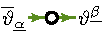
\includegraphics{appendix/diagrams/SU2model0d-Gamma2tbt.pdf}}\end{gathered}&&= -\FScoupling{m}{0}{\sigma} \suIItij{0}{\underline{\alpha}}{\underline{\beta}}-2 \iu\vts \FScoupling{Y}{0}{\sigma}\suIItij{3}{\underline{\alpha}}{\underline{\beta}}\,,\\
\FSvertexArg{\FSeaaEoM}{{\vartheta} \text{}^{\underline{\alpha}},\overline{\vartheta} {}_{\underline{\beta}}}&\equiv\begin{gathered}\raisebox{-3pt}{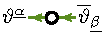
\includegraphics{appendix/diagrams/SU2model0d-Gamma2ttb.pdf}}\end{gathered}&&= \FScoupling{m}{0}{\sigma} \suIItij{0}{\underline{\beta}}{\underline{\alpha}}+2 \iu\vts \FScoupling{Y}{0}{\sigma}\suIItij{3}{\underline{\beta}}{\underline{\alpha}}\,,\\
\FSvertexArg{\FSeaaEoM}{{\pi} {}_{\underline{j}},{\pi} {}_{\underline{i}}}&\equiv \begin{gathered}\raisebox{-3pt}{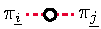
\includegraphics{appendix/diagrams/SU2model0d-Gamma2pp.pdf}}\end{gathered} &&= \delta_{\underline{i},\underline{j}} \tfrac{\FScoupling{U}{1}{\sigma}}{\sigma } = \delta_{\underline{i},\underline{j}} \tfrac{u(t,\sigma)}{\sigma}  \, , \\ 
\FSvertexArg{\FSeaaEoM}{\sigma,\sigma}&\equiv \begin{gathered}\raisebox{-3pt}{
\includegraphics{appendix/diagrams/SU2model0d-Gamma2ss.pdf}}\end{gathered} &&=\FScoupling{U}{2}{\sigma} = \partial_\sigma u(t,\sigma)\,.
\end{alignat}
\end{subequations}

The regulator insertions are given by
\begin{subequations}\label{eq:SU20ddtR}
\begin{alignat}{2}
-\partial_t\FSregulatorArg{\FSREoM}{\overline{\vartheta} {}_{\underline{\alpha}},{\vartheta} \text{}^{\underline{\beta}}} &\equiv\begin{gathered}\raisebox{-3pt}{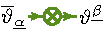
\includegraphics{appendix/diagrams/SU2model0d-Rtbt.pdf}}\end{gathered}&&= \partial_t r_f(t) \suIIIdij{\underline{\alpha}}{\underline{\beta}} = 2\partial_t r_f(t) \suIItij{0}{\underline{\alpha}}{\underline{\beta}}\, ,\label{eq:SU20ddtRtbt}\\
-\partial_t\FSregulatorArg{\FSREoM}{{\vartheta} \text{}^{\underline{\alpha}},\overline{\vartheta} {}_{\underline{\beta}}} &\equiv\begin{gathered}\raisebox{-3pt}{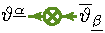
\includegraphics{appendix/diagrams/SU2model0d-Rttb.pdf}}\end{gathered}&&= -\partial_t r_f(t) \suIIIdij{\underline{\beta}}{\underline{\alpha}}= -2\partial_t r_f(t) \suIItij{0}{\underline{\beta}}{\underline{\alpha}}\, ,\label{eq:SU20ddtRttb}\\
\partial_t\FSregulatorArg{\FSREoM}{{\pi} {}_{\underline{j}},{\pi} {}_{\underline{i}}}&\equiv \begin{gathered}\raisebox{-3pt}{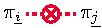
\includegraphics{appendix/diagrams/SU2model0d-Rpp.pdf}}\end{gathered} &&= \delta_{\underline{i},\underline{j}} \partial_t r_b(t) \, , \\ 
\partial_t\FSregulatorArg{\FSREoM}{\sigma,\sigma}&\equiv \begin{gathered}\raisebox{-3pt}{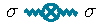
\includegraphics{appendix/diagrams/SU2model0d-Rss.pdf}}\end{gathered} &&=\partial_t r_b(t)\,,
\end{alignat}
\end{subequations}
where we introduced a minus sign for the \gmv{} insertions such that diagrams with \gmv{} regulator insertions appear with their more conventional minus sign.
We discussed this in \cref{paragraph:0dSU2flowU} following \cref{eq:Rflip}.

Recall \cref{eq:GkabImplicit}:
\begin{align}
	\FSpropagator{\FSidx{a},\FSidx{m}}[\FSmf{\FSsf}] \del{\FSvertex{\FSidx{m},\FSidx{b}}[\FSmf{\FSsf}]+\FSregulator{\FSidx{m},\FSidx{b}}}&= \FSgud{b}{a} = \FSc{\FSidx{a},\FSidx{b}}\FSd{a}{b}\, ,  \label{eq:GkabImplicitApp}
\end{align}
with which we can derive the propagators 
\begin{subequations}\label{eq:SU20dG}
\begin{alignat}{2}
\FSpropagatorArg{\FSGEoM}{\overline{\vartheta} {}_{\underline{\alpha}},{\vartheta} \text{}^{\underline{\beta}}} &=\begin{gathered}\raisebox{-3pt}{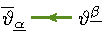
\includegraphics{appendix/diagrams/SU2model0d-Gtbt.pdf}}\end{gathered}&&= 
\frac{-(\FScoupling{m}{0}{\sigma}+2r_f(t)) \suIItij{0}{\underline{\beta}}{\underline{\alpha}}+2 \iu\vts \FScoupling{Y}{0}{\sigma}\suIItij{3}{\underline{\beta}}{\underline{\alpha}}}{\FScoupling{Y}{0}{\sigma}^2+(r_f(t)+\FScoupling{m}{0}{\sigma}/2)^2}\, ,\\
\FSpropagatorArg{\FSGEoM}{{\vartheta} \text{}^{\underline{\alpha}},\overline{\vartheta} {}_{\underline{\beta}}} &=\begin{gathered}\raisebox{-3pt}{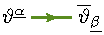
\includegraphics{appendix/diagrams/SU2model0d-Gttb.pdf}}\end{gathered}&&=
\frac{(\FScoupling{m}{0}{\sigma}+2r_f(t)) \suIItij{0}{\underline{\alpha}}{\underline{\beta}}-2 \iu\vts \FScoupling{Y}{0}{\sigma}\suIItij{3}{\underline{\alpha}}{\underline{\beta}}}{\FScoupling{Y}{0}{\sigma}^2+(r_f(t)+\FScoupling{m}{0}{\sigma}/2)^2}\, ,\\
\FSpropagatorArg{\FSGEoM}{{\pi} {}_{\underline{j}},{\pi} {}_{\underline{i}}}&= \begin{gathered}\raisebox{-3pt}{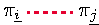
\includegraphics{appendix/diagrams/SU2model0d-Gpp.pdf}}\end{gathered} &&= \frac{1}{r_b(t)+u(t,\sigma)/\sigma} \delta_{\underline{i},\underline{j}}\, , \\ 
\FSpropagatorArg{\FSGEoM}{\sigma,\sigma}&= \begin{gathered}\raisebox{-3pt}{
\includegraphics{appendix/diagrams/SU2model0d-Gss.pdf}}\end{gathered} &&= \frac{1}{r_b(t)+\partial_\sigma u(t,\sigma)}\,,
\end{alignat}
\end{subequations}
by inverting
\begin{align}
	\big(\FSvertexArg{\FSeaEoM}{\FSidx{a},\FSidx{b}}+\FSregulatorArg{\FSREoM}{\FSidx{a},\FSidx{b}}\big)=\big(\FSvertexArg{\FSeaEoM}{\FSidx{a},\FSidx{b}}\big),
\end{align}
and carefully keeping track of the sign factors $\FSc{\FSidx{a},\FSidx{b}}$ for the Grassmann numbers.
Note that
\begin{subequations} 
\begin{align}
\big(\FSpropagatorArg{\FSGEoM}{\overline{\vartheta},{\vartheta}}\big){}^{\underline{\beta}}{}_{\underline{\alpha}}
+\big(\FSpropagatorArg{\FSGEoM}{{\vartheta},\overline{\vartheta}}\big){}^{\underline{\alpha}}{}_{\underline{\beta}} = 0\, ,\\
\big(\FSregulatorArg{\FSREoM}{{\vartheta} ,\overline{\vartheta}}\big){}^{\underline{\beta}}{}_{\underline{\alpha}}
+\big(\FSregulatorArg{\FSREoM}{\overline{\vartheta} ,{\vartheta} }\big){}^{\underline{\alpha}}{}_{\underline{\beta}} = 0\, ,
\end{align}
\end{subequations}
\ie{}, they are directly related by transposition.
This usually allows for a unification of \gmv{} contributions in the traces of the Wetterich equation, \viz{} the elimination of one class of propagators and insertions in favor of the other one, \cf{} \cref{eq:SU2model0dUFlow1,eq:SU2model0dUFlow2} in \cref{paragraph:0dSU2flowU}.
We will usually eliminate $\FSpropagatorArg{\FSGEoM}{\overline{\vartheta} {}_{\underline{\alpha}},{\vartheta} \text{}^{\underline{\beta}}}$ in favor of $\FSpropagatorArg{\FSGEoM}{{\vartheta} \text{}^{\underline{\alpha}},\overline{\vartheta} {}_{\underline{\beta}}}$ by transposition (and by using the invariance of the involved traces under such an operation).
For complicated diagrams, like the box-diagrams in the flow equation \eqref{eq:SU2model0dhFlow} for $g_t(\sigma)$, such a simple elimination by transposition is not possible while maintaining the simple order of elements on the loop, \cf{} ref a mixed diagram, and we maintain diagrams and expressions involving both propagator types.

The flow \cref{eq:SU2model0dG2tbt} for the Grassmann-valued two-point function includes the following three- and four-point vertices,
\begin{alignat}{2}
\FSvertexArg{\FSeaaEoM}{\overline{\vartheta} {}_{\underline{\beta}},{\vartheta} \text{}^{\underline{\alpha}},{\pi} {}_{\underline{i}}}&\equiv\begin{gathered}\raisebox{-6pt}{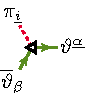
\includegraphics{appendix/diagrams/SU2model0d-V1110.pdf}}\end{gathered}&&=-2 \iu\vts  \tfrac{\FScoupling{Y}{0}{\sigma}}{\sigma } \suIItij{\underline{i}}{\underline{\beta}}{\underline{\alpha}}\, , \\ 
\FSvertexArg{\FSeaaEoM}{\overline{\vartheta} {}_{\underline{\beta}},{\vartheta} \text{}^{\underline{\alpha}},\sigma}&\equiv\begin{gathered}\raisebox{-6pt}{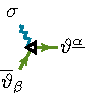
\includegraphics{appendix/diagrams/SU2model0d-V1101.pdf}}\end{gathered}&&=-\FScoupling{m}{1}{\sigma} \suIItij{0}{\underline{\beta}}{\underline{\alpha}}-2 \iu\vts \FScoupling{Y}{1}{\sigma} \suIItij{3}{\underline{\beta}}{\underline{\alpha}}\, , \\ 
\FSvertexArg{\FSeaaEoM}{\overline{\vartheta} {}_{\underline{\delta}},{\vartheta} \text{}^{\underline{\gamma}},\overline{\vartheta} {}_{\underline{\beta}},{\vartheta} \text{}^{\underline{\alpha}}}&\equiv\begin{gathered}\raisebox{-6pt}{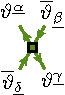
\includegraphics{appendix/diagrams/SU2model0d-V2200.pdf}}\end{gathered}&&=\FScoupling{g}{0}{\sigma} \big[\suIItij{0}{\underline{\beta}}{\underline{\alpha}} \suIItij{0}{\underline{\delta}}{\underline{\gamma}}-\suIItij{0}{\underline{\beta}}{\underline{\gamma}} \suIItij{0}{\underline{\delta}}{\underline{\alpha}}\big]\, , \\ 
\FSvertexArg{\FSeaaEoM}{\overline{\vartheta} {}_{\underline{\beta}},{\vartheta} \text{}^{\underline{\alpha}},{\pi} {}_{\underline{j}},{\pi} {}_{\underline{i}}}&\equiv\begin{gathered}\raisebox{-6pt}{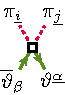
\includegraphics{appendix/diagrams/SU2model0d-V1120.pdf}}\end{gathered}&&=-\delta_{\underline{i},\underline{j}} \Big[\tfrac{\FScoupling{m}{1}{\sigma}}{\sigma }\suIItij{0}{\underline{\beta}}{\underline{\alpha}}+2 \iu \vts\partial_{\sigma}\Big(\tfrac{\FScoupling{Y}{0}{\sigma}}{\sigma }\Big) \suIItij{3}{\underline{\beta}}{\underline{\alpha}}\Big]\, , \\ 
\FSvertexArg{\FSeaaEoM}{\overline{\vartheta} {}_{\underline{\beta}},{\vartheta} \text{}^{\underline{\alpha}},\sigma,\sigma}&\equiv\begin{gathered}\raisebox{-6pt}{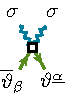
\includegraphics{appendix/diagrams/SU2model0d-V1102.pdf}}\end{gathered}&&=-\FScoupling{m}{2}{\sigma}\suIItij{0}{\underline{\beta}}{\underline{\alpha}}-2 \iu \vts\FScoupling{Y}{2}{\sigma} \suIItij{3}{\underline{\beta}}{\underline{\alpha}}\, ,
\end{alignat}
while the flow equation for the Grassmann-valued four-point function in \cref{paragraph:0dSU2flowh} includes, furthermore, the following mixed four-, five-, and six-point vertices,
\begin{alignat}{2}
\FSvertexArg{\FSeaaEoM}{\overline{\vartheta} {}_{\underline{\beta}},{\vartheta} \text{}^{\underline{\alpha}},{\pi} {}_{\underline{i}},\sigma}&\equiv\begin{gathered}\raisebox{-6pt}{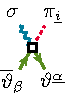
\includegraphics{appendix/diagrams/SU2model0d-V1111.pdf}}\end{gathered}&&=-2 \iu \vts \partial_{\sigma}\Big(\tfrac{\FScoupling{Y}{0}{\sigma}}{\sigma }\Big) \suIItij{\underline{i}}{\underline{\beta}}{\underline{\alpha}}\, , \\ 
\FSvertexArg{\FSeaaEoM}{\overline{\vartheta} {}_{\underline{\delta}},{\vartheta} \text{}^{\underline{\gamma}},\overline{\vartheta} {}_{\underline{\beta}},{\vartheta} \text{}^{\underline{\alpha}},\sigma}&\equiv\begin{gathered}\raisebox{-6pt}{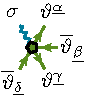
\includegraphics{appendix/diagrams/SU2model0d-V2201.pdf}}\end{gathered}&&=\FScoupling{g}{1}{\sigma} \big[\suIItij{0}{\underline{\beta}}{\underline{\alpha}} \suIItij{0}{\underline{\delta}}{\underline{\gamma}}-\suIItij{0}{\underline{\beta}}{\underline{\gamma}} \suIItij{0}{\underline{\delta}}{\underline{\alpha}}\big]\, , \\ 
\FSvertexArg{\FSeaaEoM}{\overline{\vartheta} {}_{\underline{\delta}},{\vartheta} \text{}^{\underline{\gamma}},\overline{\vartheta} {}_{\underline{\beta}},{\vartheta} \text{}^{\underline{\alpha}},{\pi} {}_{\underline{j}},{\pi} {}_{\underline{i}}}&\equiv\begin{gathered}\raisebox{-6pt}{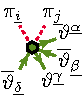
\includegraphics{appendix/diagrams/SU2model0d-V2220.pdf}}\end{gathered}&&=\delta_{\underline{i},\underline{j}} \tfrac{\FScoupling{g}{1}{\sigma}}{\sigma } \big[\suIItij{0}{\underline{\beta}}{\underline{\alpha}} \suIItij{0}{\underline{\delta}}{\underline{\gamma}}-\suIItij{0}{\underline{\beta}}{\underline{\gamma}} \suIItij{0}{\underline{\delta}}{\underline{\alpha}}\big]\, , \\ 
\FSvertexArg{\FSeaaEoM}{\overline{\vartheta} {}_{\underline{\delta}},{\vartheta} \text{}^{\underline{\gamma}},\overline{\vartheta} {}_{\underline{\beta}},{\vartheta} \text{}^{\underline{\alpha}},\sigma,\sigma}&\equiv\begin{gathered}\raisebox{-6pt}{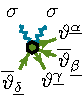
\includegraphics{appendix/diagrams/SU2model0d-V2202.pdf}}\end{gathered}&&=\FScoupling{g}{2}{\sigma} \big[\suIItij{0}{\underline{\beta}}{\underline{\alpha}} \suIItij{0}{\underline{\delta}}{\underline{\gamma}}-\suIItij{0}{\underline{\beta}}{\underline{\gamma}} \suIItij{0}{\underline{\delta}}{\underline{\alpha}}\big]\,.
\end{alignat}

\renewcommand{\FSk}{k}